\let\textcircled=\pgftextcircled
\chapter{Preliminaries}
\label{chap:prelim}


\bigskip

\section{Mathematical background of quantum theory}

\subsection{Hilbert space theory}

We will be considering separable Hilbert spaces over the complex numbers, where separability is taken to mean the existence of a countable orthonormal basis. We will adopt the convention that the inner product, denoted $\langle\cdot|\cdot\rangle$, is linear in the second argument and conjugate-linear in the first. Such an inner product naturally induces a norm $\norm{\boex} \defeq \sqrt{\langle \boex| \boex\rangle}$. We will use the notation $\bops[V][W]$ for the space of continuous (and equivalently bounded) linear maps between normed vector spaces $V$ and $W$, over the same field, omitting the second argument if the two spaces are the same. This set is once more a vector space over the same field, with addition and scalar multiplication being defined pointwise. Moreover it inherits a natural norm, called the \emph{operator norm} 
\begin{align}
  \norm{\cdot}&:\bops[V][W]\to \K\\
  \norm{T} &\defeq \sup_{\substack{\bov\in V \\ \norm{\bov}\leq 1}}\norm{T\bov}, \label{eqn:operator-norm}
\end{align}
under which it is a Banach space. A particularly important special case is the space of maps $\bops[V][\K]$, where $\K$ is the field underlying $V$, which we will denote $V^*$, and is commonly called the topological dual of $V$. A celebrated theorem due to Riesz \cite{riesz-representation-riesz} and Fr{\'e}chet \cite{riesz-representation-frechet}, commonly called the Riesz representation theorem, states that Hilbert space over $\R$ is isomorphic to its topological dual, and one over $\Cx$ is anti-isomorphic to its dual. More explicitly every continuous linear functional on a Hilbert space is of the form $\Psi_{\bow} :\bov\mapsto \langle{\bow} |\bov\rangle$, for some fixed $\bow\in V$, and the map $\Psi_{\bow}$, defined in this way is a continuous linear functional for every $\bow\in V$.

% Given two vector spaces, $V$, $W$ over the same field $\K$ we define the \emph{tensor product} $V\times W$ by first defining the free vector space over $\K$, $F(V\otimes W)$ generated by the tuples $(\bov, \bow)$ for each $\bov\in V$ and $\bow\in W$. To obtain the tensor product we then quotient by the equivalence relation $\sim$ such that
% \begin{align}
%   (\bov,\bow) + (\bov^\prime, \bow) &\sim (\bov+ \bov^\prime, \bow)\\
%   (\bov,\bow) + (\bov, \bow^\prime) &\sim (\bov, \bow+\bow^\prime)\\
%   c(\bov,\bow) &\sim (c\bov,\bow)\sim (\bov,c\bow),
% \end{align}
% for all $\bov, \bov^\prime\in V$, $\bow,\bow^\prime \in W$, $c\in \K$. We denote the equivalence class $[(\bov,\bow)]$ by $\bov\otimes \bow$.

% We define the \emph{tensor product} $V\otimes W$ of two vector spaces $V$ and $W$ abstractly to be the quotient of the free vector space generated by the symbols $\bov\otimes \bow$, for all $\bov\in V$ and $\bow\in W$, by the relations. We note that if $\hcal$ and $\kcal$ are inner product spaces we may define an inner product on $\hcal\otimes\kcal$ by 
% \begin{align}
%   \langle \phi_1\otimes \psi_1 | \phi_2\otimes \psi_2\rangle = \langle \phi_1 | \phi_2\rangle \langle \psi_1 | \psi_2\rangle,
% \end{align}
% and extending linearly to the whole space. If $V$ and $W$ are Hilbert spaces then $V\otimes W$, with $\otimes$ defined in this way is not generally a Hilbert space, because it is not complete. For Hilbert $\hcal$ and $\kcal$ spaces we call take the completion with respect to the inner product defined above to get $\hcal\otimes\kcal$. As we shall see later, once we have defined the trace of an operator, there is relatively explicit construction of the tensor product of Hilbert spaces in terms of the Hilbert-Schmidt class of operators.

We are often required to consider maps which are not defined on the whole Hilbert space. An \emph{operator} is a linear map $A$ whose domain, denoted $D(A)$, is a vector subspace (not necessarily closed) of the Hilbert space of interest. A motivating example is the differential operator $\opp:\phi\mapsto -i \phi^\prime$, defined on the subspace of absolutely continuous functions in $L^2(\R)$, whose weak derivatives are also in $L^2(\R)$. If $A:\hcal\to\kcal$ is an operator, defined on a dense domain $D(A)\subseteq \hcal$ we may define the domain of the \emph{adjoint} $D(A^*)$, to be the set of vectors $\psi \in \kcal$ for which there exists an $\eta_{\psi}\in \hcal$ such that
\begin{align}
  \langle \psi | A\phi \rangle  = \langle \eta_{\psi}| \phi\rangle,
\end{align}
holds for all $\phi\in D(A)$. We then define $A^*$ on this domain to be
\begin{align}
  A^* \psi = \eta_{\psi},
\end{align}
noting that the density of $D(A)$ ensures that the element $\eta_{\psi}$ is unique, for those $\psi$ for which it exists. For $\bops[\hcal]$ the situation is somewhat simpler, the domain of $A$ and $A^*$ can both be taken to be $\hcal$. In this case the map $A\mapsto A^*$ is a conjugate linear isomorphism preserving the operator norm \eqref{eqn:operator-norm}, and the equations
\begin{align}
  (AB)^* &= B^* A^*\\
  A^{**} &= A\\
  \left(A^{-1}\right)^* &= \left(A^*\right)^{-1},
\end{align}
hold, with the last equation requiring the additional assumption that $A$ is invertible with bounded inverse. 

The \emph{compact operators} are an important subclass of the bounded operators, they are those which may be written as the limit of a sequence of finite rank operators
\begin{align}
  T_n:\varphi&\mapsto\sum_{k=0}^n \lambda_k\braket{f_k}{\varphi} \ket{g_k} \\
  T_n &\xrightarrow{n\to\infty} T,
\end{align}
where the limit converges in the operator norm and $(f_k)_{k\in \N}$ and $(g_k)_{k\in \N}$ are orthonormal sets in $\hcal$.

Certain operators are equal to their own adjoint, we call those \emph{self-adjoint}, denoted $\saops[\hcal]$, and note that they form a vector space over the reals, where the domain of a sum of two operators is the intersection of the domains. 

Those operators which may be written in the form $A = B^*B$, for some operator $B$ are called positive, we denote this with $A\geq 0$. The set of such operators forms a \emph{convex  cone} in $\saops[\hcal]$ (see section \ref{sec:prelim-comvex-analysis}, for definitions related to convexity) denoted $\posops[\hcal]$. For any $\psi\in D(A^*A)$ we have that 
\begin{align}
  \langle\psi | B^* B \psi \rangle &= \langle B \psi | B \psi\rangle \\
                                  &= \norm{B\psi}^2 \geq 0.
\end{align}
There is a natural a partial order on the space $\saops[\hcal]$: defined via $\posops[\hcal]$, we will say $A\geq B$, iff $A-B\geq 0$. Every positive operator $A$ has a square root, the unique positive operator $B$ such that $A = B^2$; this may be shown via the spectral theorem, although independent proofs also exist.


We define the operator absolute value to be
\begin{align}
  \abs{A} \defeq \sqrt{A^*A},
\end{align}
noting that $A^*A$ and $\abs{A}$ are bounded if and only if $A$ is.

If $\seq{\boe_k}[k\in\N]$ is an orthonormal basis for a Hilbert space $\hcal$ then we define the trace of an operator $A\in\bops[\hcal]$ by
\begin{align}
  \tr{A} &= \sum_k \braket{\boe_k}{A\boe_k},
\end{align}
however this quantity is not, in general, independent of the basis chosen, even if it is finite, see appendix \ref{app:bad-sum-is-bad} for an example. We consider the restricted class of operators such that
\begin{align}
  \sum_k \braket{\boe_k}{\left(\abs{A}\boe_k}\right),
\end{align}
converges to some real number for any, equivalently every, basis $\seq{\boe_k}[k\in\N]$. We call these operators \emph{trace-class}, denoted $\trops[\hcal]$. For elements of $\trops[\hcal]$ the infinite sum
\begin{align}
  \tr{A} &= \sum_k \braket{\boe_k}{A\boe_k},
\end{align}
is \emph{absolutely convergent}, and is independent of the choice of basis. Every trace-class operator is bounded, and compact. The trace-class operators form a vector space over $\Cx$, we summarise several useful properties in Lemma \ref{lem:properties-of-trops}.
\begin{lem}[Properties of the trace-class]
\label{lem:properties-of-trops}\leavevmode
\begin{itemize}
  \item the trace is a linear functional on $\trops[\hcal]$,
  \item the map $(A, B)\mapsto \tr{A^*B}$ is an inner product on $\trops[\hcal]$,
  \item the map $A\mapsto \sqrt{\tr{A^*A}}$ is a norm on $\trops[\hcal]$, called the Hilbert-Schmidt norm and denoted $\norm{A}_{\text{HS}}$,
  \item $\tr{A^*} = \tr{A}^*$,
  \item if $A$ is trace-class and $B$ is bounded then $AB$ and $BA$ are trace-class, hence $\trops[\hcal]$ is a two-sided ideal in the bounded operators,
  \item further, the vector-space of maps on the trace-class of the form $A\mapsto\tr{AB}$, where $B$ is bounded is the topological dual of the trace-class.
\end{itemize}
\end{lem}
Given two Hilbert spaces $\hcal$ and $\kcal$ there is a Hilbert space $\hcal_\otimes$ and a bilinear map $f:\hcal\times\kcal\to\hcal_\otimes$ such that the subspace $\vspan{\sbuild{f(\phi,\psi)}{\phi\in\hcal, \psi\in\kcal}}$ is dense in $\hcal_\otimes$ and 
$\braket{f(\phi_1,\psi_2)}{f(\phi_2,\psi_2)} = \braket{\phi_1}{\phi_2}\braket{\psi_1}{\psi_2}$ for all $\phi_1,\phi_2\in\hcal$ and $\psi_1,\psi_2\in\kcal$. We write $\hcal_\otimes =: \hcal\otimes\kcal$, called the \emph{tensor product} of $\hcal$ and $\kcal$, since it is unique up to isomorphism. Given $S\in\bops[\hcal]$ and $V\in\bops[\kcal]$ there exists a unique operator, $S\otimes T\in\bops[\hcal\otimes\kcal]$ such that 
\begin{align}
  (S\otimes T)(\phi\otimes\psi) = (S\phi)\otimes(T\psi),
\end{align}
holds for all $\phi\in\hcal$ and $\psi\in\kcal$. We call  $(S\otimes T)$ the tensor product of $S$ and $T$ and note some fundamental properties in lemma \ref{lem:properties-of-tensor}.
\begin{lem}[Properties of the operator tensor product]\label{lem:properties-of-tensor}\leavevmode
\begin{itemize}
  \item $\alpha(S\otimes T) = (\alpha S)\otimes T = S\otimes(\alpha T)$, for all $\alpha\in\Cx$,
  \item $(S_1 + S_2)\otimes T = S_1\otimes T + S_2 \otimes T$,
  \item $(S_1\otimes T_1)(S_2\otimes T_2) = S_1S_2 \otimes T_1 T_2$,
  \item $(S\otimes T)^* = S^*\otimes T^*$,
  \item if $S$ and $T$ are both self-adjoint, unitary, positive or trace-class then so is $S\otimes T$ respectively,
  \item $\tr{S\otimes T} = \tr{S}\tr{T}$.
\end{itemize}
\end{lem}
A partial inverse of the tensor product is the so-called \emph{partial trace}: if $T\in\trops[\hcal\otimes\kcal]$ then there is a unique $T_1\in\trops[\hcal]$ such that
\begin{align}
  \tr{T_1 A} = \tr{T(A\otimes \opi_\kcal)},
\end{align}
holds for all $A\in \bops[\hcal]$. The partial trace is linear, and trace-preserving. It is also positive, in the sense that it maps positive operators to positive operators and completely positive in the sense of definition \ref{defn:completely-positive-map}.

\begin{defn}\label{defn:c-star-algebra}
  A subset $\acal$ of the algebra of bounded operators on a Hilbert space is a $C^*$-algebra if it is
  \begin{itemize}
    \item Closed under the operator product $a,b\in\acal\implies ab\in\acal$,
    \item Closed under the operator sum $a,b\in\acal\implies a+b\in\acal$
    \item Closed under multiplication by complex numbers $a\in\acal, \alpha\in\Cx \implies \alpha a \in \acal$
    \item Closed under taking adjoints: $a\in\acal \implies a^*\in\acal$
    \item Closed in the  topology induced by the operator norm
  \end{itemize}
\end{defn}

We note that this definition is somewhat nonstandard, a  $C^*$-algebra may also be defined as an abstract algebra obeying certain assumptions. However the Gelfand-Naimark theorem~\cite{gelfand-naimark-1943} shows that all abstract $C^*$-algebras are isometrically $*$-isomorphic to some $C^*$-subalgebra of the bounded operators on a Hilbert space. There is, therefore, no loss of generality in taking definition \ref{defn:c-star-algebra}.

% \begin{defn}\label{defn:c-star-algebra}
%   A \emph{$C^*$-algebra} is an algebra $\acal$, together with a norm $\norm{\cdot}:\acal\to\R$, and a map $\cdot^*:\acal\to\acal$ with the following properties
%   \begin{itemize}
%     \item $(\acal, \norm{\cdot})$ form a Banach algebra,
%     \item $*$ is an involution: $\left(a^*\right)^* = a$,
%     \item $(a+b)^* = a^* + b^*$,
%     \item $(ab)^* = b^* a^*$,
%     \item $\left(\alpha a\right) = \alpha^* a^*$,
%     \item $\norm{xy} \leq \norm{x}\norm{y}$,
%     \item $\norm{a^* a} = \norm{a^*}\norm{a}$.
%   \end{itemize}
% \end{defn}

\begin{defn}\label{defn:completely-positive-map}
  A map $\Phi:\acal\to \bops[\kcal]$, where $\acal\subseteq \bops[\hcal]$ is a $C^*$-algebra is $k$-positive if the induced map
  \begin{align}
    \operatorname{id}_k\otimes \Phi:\Cx^{k\times k}\otimes \acal\to \Cx^{k\times k}\otimes\bops[\kcal]
  \end{align}
  is positive, and $\Phi$ is \emph{completely positive} if it is $k$-positive for all $k\in\N$.
\end{defn}

\begin{thm}[Stinespring]\label{thm:stinespring}
  Let $\Phi:A\to\bops[\kcal]$ be a completely positive map, where $A\subseteq\bops[\hcal]$ is a $C^*$ algebra, then $\Phi$ is completely positive if and only if it admits the representation
  \begin{align}
    \Phi(X) = V^* \pi(X) V,
  \end{align}
  where $V:\kcal\to\kcal^\prime$ is a a bounded linear map, $\kcal^\prime$ is a Hilbert space and $\pi$ is a $*$-homomorphism\footnote{A homomorphism of algebras, each equipped with an involution $*$, such that $\pi(a^*)=\pi(a)^*$.} of $A$ in $\bops[\tilde{\kcal}]$.
\end{thm}

Of particular interest for applications in quantum theory are the completely positive maps between spaces of trace-class operators which preserve the trace. Recalling that the dual of the trace-class is the space of bounded operators we can define the dual of a trace-preserving completely positive map by requiring that
\begin{align}
  \tr{A \Phi(B)} = \tr{\Phi^*(A) B},
\end{align}
for all $A\in\bops[\hcal]$ and $B\in\trops[\hcal]$. The dual of a trace-preserving completely positive map is again completely positive and is \emph{unital} $\Phi^*(\opi) = \opi$ and \emph{normal} in the sense that
\begin{align}
  X_a \uparrow X \implies \Phi^*(X_a) \uparrow \Phi(X),
\end{align}
where $\uparrow$ denotes the increasing limit. For detailed information on Stinespring's theorem and the properties of positive and completely positive maps see e.g. \cite{stormer1963} and \cite{stormer1974}.

\subsection{Measures and operator valued measures}

Let $\Omega$ be a set and $\fcal$ a subset of the power set of $\Omega$ which includes the empty set, is closed under complements and is closed under countable unions. A set with these properties is called a \emph{$\sigma$-algebra} on $\Omega$, and an ordered pair $(\Omega, \fcal)$ of set and $\sigma$-algebra of subsets is called a \emph{measurable space}. A (positive, extended real) \emph{measure} on $(\Omega, \fcal)$ is a function $\mu$ from $\fcal$ to $\R\cup \{\infty\}$ such that
\begin{itemize}
  \item $\forall S\in\fcal $, $\mu(S)\geq 0$,
  \item There exists a set $S\in\fcal$ such that $\mu(S) \in\R$,
  \item If $\seq{S_k}[k\in\N]$ is a countable sequence of non-intersecting sets in $\fcal$, then $\mu(\bigcup_k S_k) = \sum_k\mu(S_k)$,
\end{itemize}
From these properties it immediately follows that $\mu(\varnothing) = 0$, as $\mu(S) = \mu(S \cup \varnothing\cup\varnothing\ldots) = \mu(S) + \mu(\varnothing) + \mu(\varnothing)\ldots$. We define general extended real, and complex measures in the obvious way: an extended real measure $\mu$ is a pair of positive measures $\mu_\pm$ such that $\mu(S) = \mu_+(S) - \mu_-(S)$, and a complex measure may be defined by its real and imaginary parts. A positive measure such that $\mu(\Omega) = 1$ is called a probability measure, and we denote the set of probability measures on $(\Omega,\fcal)$ by $\probs{\Omega}{\fcal}$. If $\Omega$ has a topology $\tau$ then the Borel $\sigma$-algebra, denoted $\borel{\Omega}[\tau]$, or $\borel{\Omega}$, where there is no possibility of confusion, is the smallest $\sigma$-algebra containing the open sets of $\tau$. The elements of $\borel{\Omega}$ are called the Borel sets. All of the probability measures we encounter in this thesis will be Borel, either with respect to the standard topology on the reals or the topology generated by the singleton sets where $\Omega$ is finite.

It is essential for the development of the spectral theory of self adjoint operators to consider ``measures'' which map into (subsets of) the bounded operators on some Hilbert space.

\begin{defn}[Positive operator valued measure]\label{defn:povm}
  A positive operator valued measure (POVM) on a set $\Omega$ with $\sigma$-algebra $\fcal$ is a function $E:\fcal\to\posops[\hcal]$ such that $E(\Omega) = \opi$ and for all sequences of non-intersecting sets in $\fcal$ $\seq{S_k}[k\in\N]$ we have 
  \begin{align}
    E\left(\bigcup_k \,S_k\right) = \sum_k E(S_k).
  \end{align}
\end{defn}
We note that one can show that the effects (often called POVM elements) $\sbuild{E(S)}{S\in\fcal}$ are bounded operators, in particular $\norm{E(S)\varphi} \leq \norm{E(\Omega)\varphi} = \norm{\varphi}$. We will often be interested in the case where a POVM is a projection valued measure (PVM), in the sense that $E(S)^2 = E(S)$, for all $S\in\fcal$. Equivalent to this definition is a multiplicative property $E(S)E(T) = E(S\cap T)$, for all $S,T\in\fcal$. Given a Borel PVM $E_A$ over the reals, there is a vector subspace $D(A)\subseteq\hcal$ such that the integral
\begin{align}
  \int_\R x d\braket{\psi}{E_A(x)\phi} 
\end{align}
converges for all $\psi,\phi\in D(A)$, and a unique self-adjoint operator $A$ with domain $D(A)$ such that 
\begin{align}
  \braket{\psi}{A\phi} = \int_\R x dE_a(x),
\end{align}
for $\psi$, $\phi$ in the domain.

We give several versions of the spectral theorem, the first of which is the converse of the above statement.

\begin{thm}[Spectral theorem for self-adjoint operators]
  If $\opa$ is a self-adjoint operator with dense domain $D(A)$, then there is a unique PVM $E_A$ such that
  \begin{align}
    \braket{\psi}{A\phi} = \int_\R x d\braket{\psi}{E_A(x)\phi},
  \end{align}
  holds for all $\psi,\phi\in D(A)$.
\end{thm}

\begin{thm}[Spectral theorem for self-adjoint operators - bounded functional calculus]\label{thm:spectral-sa-ops-bounded-functions}
    Let $A$ be a self-adjoint operator on $\hcal$, there is a unique map $\hat{\phi}$ from the bounded Borel functions on $\R$ to $\bops[\hcal]$ such that
    \begin{itemize}
      \item $\hat{\phi}$ is an algebraic $*$-homomorphism,
      \item $\hat{\phi}$ is norm continuous $\norm{\hat{\phi}(h)} \leq \norm{h}_\infty$,
      \item if $h_n$ is a sequence of bounded Borel functions converging (pointwise) to the identity function and $\abs{h_n(x)} \leq x$ for all $x$ and $n$, then for any $\psi\in D(A)$ we have $\lim_{n\to\infty} \hat{\phi}(h_n)\psi = A\psi$,
      \item if $h_n \to h$ pointwise and the sequence $\norm{h_n}_\infty$ is bounded then $\hat{\phi}(h_n) \to \hat{\phi}(h)$ strongly,
      \item if $A\psi$ = $\lambda\psi$ then $\hat{\phi}(h)\psi = h(\lambda)\psi$,
      \item if $h\geq 0$ then $\hat{\phi}(h) \geq 0$.
    \end{itemize}
\end{thm}

We use this as a stepping stone to a more general formulation.

\begin{thm}[Spectral theorem for self-adjoint operators - Borel functional calculus]\label{thm:spectral-sa-ops-unbounded-functions}
  Let $A$ be a self-adjoint operator on $\hcal$, and $\chi_\Omega$ the characteristic function of the measurable set $\Omega\subseteq\R$. We define the operators $P_\Omega = \hat{\phi}(\chi_\Omega)$, and note the properties
  \begin{itemize}
    \item the $P_\Omega$ are orthogonal projections,
    \item $P_\R = I$ and $P_\varnothing = 0$,
    \item if $\Omega$ is a countable union of disjoint sets $\Omega_n$ then $P_\Omega = \lim_{N\to\infty} \sum_{n=1}^N P_{\Omega_n}$, where the limit converges strongly,
    \item $P_\Omega P_\Delta = P_{\Omega\cap\Delta}$.
  \end{itemize}
  We call the map $E_A:\Omega\mapsto P_\Omega$ the spectral measure of $A$. The map $\Omega\mapsto\langle\psi| P_\Omega \phi\rangle$ is a complex-valued Borel measure on $\R$ for each $\psi, \phi\in\hcal$ and denote it $\mu_{\psi\phi}$. If $g$ is a bounded Borel function on $\R$ then we can define $g(A)$ by
  \begin{align}
    \langle \psi|g(A)\phi\rangle = \int_\R g(\lambda)\,d\mu_{\psi\phi}(\lambda),
  \end{align}
  and note that this agrees with $\hat{\phi}(g)$, further if $g$ is an unbounded, complex valued Borel function on $\R$ we define 
  \begin{align}
    D(g(A)) &= \sbuild{\psi}{\int_\R \abs{g(\lambda)}^2 d\mu_{\psi\psi}(\lambda)<\infty}\\
    \langle \psi | g(A)\phi\rangle &= \int_\R g(\lambda) d\mu_{\psi\phi}(\lambda).
  \end{align}
  We write $g(A) = \int_\R g(\lambda) P_\lambda$, and note that $g(A)$ is self-adjoint if $g$ is real. 
\end{thm}
We call the support of a self-adjoint operator $A$, $\supp{A}$, the complement of the union of all the open sets $\Omega$ for which $P_\Omega = 0$, and note that we can restrict the integrals over $\R$ in the previous theorem to be over $\supp{A}$; we therefore allow Borel functions defined on $\supp{A}$, rather than requiring that they are defined on the whole real line. We note that the definition of the support given here matches the \emph{spectrum} of a closed operator
\begin{align}
  \spec{A} = \Cx \setminus \res{A},
\end{align}
where the \emph{resolvant set}, $\res{A}$ is defined to be the set of $\lambda\in\Cx$ for which $\lambda I - A$ is a bijection onto $\hcal$ with a bounded inverse. For a self-adjoint operator the terms spectrum and support are interchangeable. 

Some important special cases are: the spectral measure of a compact operator is supported on a finite number of points or a sequence of points which converges to zero; the spectral measure of an operator on a finite dimensional Hilbert space is supported on a finite number of points; the spectral measure of a positive operator is supported within the non-negative real numbers.

\section{Convex analysis}
\label{sec:prelim-comvex-analysis}
Convex analysis concerns itself with convex sets and convex functions. Although there is an interesting theory of convex subsets of infinite dimensional vector spaces\footnote{See, for example \cite{10.1007/978-1-84800-155-8_12}.} this is beyond the scope of this thesis. Here all convex sets will be subsets of finite dimensional real vector spaces. We will follow the exposition of Rockafellar \cite{rtr-conv-anal-book}. Since we are only dealing with finite dimensional spaces a vector space $V$ is canonically isometrically isomorphic to its bidual $V^{**}$, and we do not distinguish the two, equating the vector $\boex\in V$ and the evaluation map $(\psi\mapsto\psi(\boex))\in V^{**}$. This identification is convenient for discussing the convex conjugate of a function.

\begin{defn}\label{defn:convex-set}
  A subset $C$ of a real vector space is \emph{convex} if for all $\boex,\boy\in C$ and for all $\lambda\in [0,1]$
  \begin{align}
    \lambda \boex + (1-\lambda)\boy\in C.
  \end{align}
\end{defn}
Examples of convex sets include
\begin{itemize}
  \item Any interval in $\R$,
  \item The balls in any normed vector space over the reals,
  \item The state-space $\dops$ of quantum mechanics, defined in Section \ref{sec:prelim-quantum},
  \item The set of points in $\R^2$ that lie ``above'' the graph of the function $x\mapsto x^2$, i.e. the set of points $\sbuild{(x,y)}{y > x^2}$.
\end{itemize}
This last example motivates the definition of a convex function
\begin{defn}\label{defn:epigraph}
  The \emph{epigraph} of a function $f:V\to\R$, where $V$ is a real vector space is the set of points in the vector space $V\oplus \R$ ``above'' the graph of $f$,
  \begin{align}
    \epi f = \sbuild{(v, \mu)}{v\in V,\, \mu\in\R, \mu \geq f(v)}.
  \end{align}
\end{defn}
\begin{defn}\label{defn:real-convex-function}
  A function from a real vector-space to the reals is \emph{convex} if its epigraph is a convex set.
\end{defn}
This definition of convexity for functions is slightly too restrictive, in the present context, since it only covers functions defined on an entire vector space $V$. We will mainly be concerned with, for example, uncertainty measures which are non-negative, and so we are motivated to find a definition of convexity appropriate for more general domains.

It is convenient to define the extended reals $\exR = \R \cup \{\infty, -\infty\}$, with the obvious axioms for extending the order relation, addition and multiplication. We also define $\inf\varnothing = \infty$ and $\sup\varnothing = -\infty$.
% \begin{defn}\label{defn:extended reals}
%   We define the \emph{extended reals} as an extension of the ordered field of real numbers $\exR = \R \cup \{\infty, -\infty\}$ with the following axioms
%   \begin{enumerate}
%     \item $\forall x\in\R$, $\infty > x$ and $-\infty < x$,
%     \item $\forall x\in\R$, $x + \infty = \infty + x = \infty$,
%     \item $\forall x\in\R$, $x + \infty = \infty + x = \infty$,
%     \item $\infty + \infty = \infty$ and $-\infty - \infty = -\infty$,
%     \item $\forall x\in\R$, $x>0 \implies x\infty = \infty x =  \infty$ and $x(-\infty) = (-\infty)x = -\infty$,
%     \item $\forall x\in\R$, $x<0 \implies x\infty = \infty x = -\infty$ and $x(-\infty) = (-\infty)x = \infty$,
%     \item $0 \infty = \infty 0 = 0 = 0(-\infty) = (-\infty)0$,
%     \item $\inf\varnothing = \infty$ and $\sup\varnothing = -\infty$.
%   \end{enumerate}
% \end{defn}
We can now consider functions defined on arbitrary convex subsets of real vector spaces, simply by extending the function to be $\infty$ outside. We note that, strictly speaking, this recourse to the extended reals is unnecessary and one can consider convex functions defined on convex subsets of real vector spaces directly, but this leads to more tedious consideration of domains. In the present formulation one can recover the domain by considering the points where the extended function takes finite values. The forms $\infty-\infty$ and $-\infty +\infty$ are left undefined, in principle it is important to be cautious about these cases, but they do not arise within this work.

For completeness we define the epigraph and convexity for extended real functions, although these are essentially identical to definitions given above.
\begin{defn}\label{defn:extended-convex-function}
  A function $f:V\to\exR$, where $V$ is a real vector space, is \emph{convex} if its epigraph
  \begin{align}
    \epi f = \sbuild{(v,\mu)}{v\in V,\,\mu\in \R,\,\mu\geq f(v)},
  \end{align}
  is a convex subset of $V\oplus R$. Note that if $f(v) =\infty$ there are no $\mu\in\R$ such that $\mu\geq f(v)$, so these $v$ do not occur in any of the ordered pairs in $\epi f$.
\end{defn}
We now state two useful theorems of convex functions.
\begin{thm}\label{thm:jensen-two-point}
  Let $f:V\to (-\infty, \infty]$, with $V$ a real vector space. Then $f$ is convex if and only if the inequality
  \begin{align}
    f(\lambda \boex + (1-\lambda)\boy) \leq \lambda f(\boex) + (1-\lambda)f(\boy)
  \end{align}
  holds for all $\boex,\boy\in V$ and $\lambda\in [0,1]$. The exception of $-\infty$ is to exclude pathological cases where $f(\boex)$ and $f(\boy)$ are different infinite values.
\end{thm}
\begin{thm}[Jensen's inequality]\label{thm:jensen-n-point}
  Let $f:V\to (-\infty, \infty]$, with $V$ a real vector space. Then $f$ is convex if and only if the inequality
  \begin{align}
    f\left( \sum_{i=1}^n \lambda_i \boex_i \right) \leq \sum_{i=1}^n\lambda_i f(\boex_i),
  \end{align}
  holds for all $\boex_i\in V$ and $\lambda_i\in [0,1]$ such that $\sum_{i=1}^{n}\lambda_i = 1$.
\end{thm}
There are also generalisations to countable sets of points, and probability measures in the uncountable case \cite{Cover:2006:EIT:1146355}\cite{PERLMAN197452}.

It is useful to define the \emph{convex conjugate} of a function, which we will apply extensively in section \ref{chap:cov-meas-ur}.

\begin{defn}\label{defn:convex conjugate}
  Given a function $f:V\to\exR$, where $V$ is a topological vector space over the reals, we define the convex conjugate of $f$ to be
  \begin{align}
    f^*&:V^*\to \exR\\
    f^*&:\boalpha\mapsto\sup_{\bov\in V} \{\langle\boalpha,\bov\rangle - f(\bov)\},
  \end{align}
  where $V^*$ is the space of continuous linear functionals on $V$ and $\langle\cdot,\cdot\rangle$ denotes the dual pairing between $V$ and $V^*$. 
\end{defn}

\begin{thm}
  The biconjugate $(f^{*})^*$ of a function $f:V\to\exR$ is the greatest (pointwise) lower-semi continuous function which is bounded above by $f$.
\end{thm}

Where $f$ is a convex function $(f^*)^*$ (hereafter denoted $f^{**}$) is equal to $f$.

\section{Semidefinite programming}
The usual formulation~\cites{Vandenberghe-Boyd-semidefinite} of semi-definite programming is in terms of $n\times n$ positive-semidefinite real matrices with real elements. Here, following the exposition given in \cite{w-semidefinite-prog-cb-norms}, we use a slightly different but entirely equivalent formulation better adapted to problems in quantum mechanics. 

\begin{defn}\label{defn:complex-semidefinite-program}
  Let $\hcal$, $\kcal$ be finite-dimensional Hilbert spaces, $\opc\in\saops[\hcal]$, $\opd\in\saops[\kcal]$ and let $\Psi:\saops[\hcal]\to\saops[\kcal]$ be a linear map. The \emph{primal semidefinite problem} and \emph{dual semidefinite problem}  associated to the triple $\left(\Psi, \opc, \opd\right)$ are
  \begin{equation}
  \begin{aligned}
    & \underset{X\in\posops[\hcal]}{\text{maximise}} & &\tr{\opc X } \qquad\qquad & & \underset{Y\in\posops[\kcal]}{\text{minimise}} & & \tr{\opd Y} \\
    & \text{subject to} & &\Psi(X) \leq \opd & & \text{subject to} & &  \Psi^*(Y) \geq C,
  \end{aligned}
  \label{eqn:semidefinite-program}
\end{equation}
respectively.
\end{defn}

Here it is traditional to note the analogy with the classical theory of linear programming,  we therefore note the duality theorem for linear programs \eqref{thm:duality-linear-prog} from ref.~\cite{schrijver-lin-int-prog}.
\begin{thm}\label{thm:duality-linear-prog}
  Let $\opa\in\R^{n\times m}$, $\boc\in\R^n$ and $\bob\in\R^m$ then
  \begin{align}
    \sup\left\{\boc\cdot \boex \middle| \boex\in\R^n,\, A \boex \leq \bob\right \} = \inf\left\{ \bob\cdot\boy \middle|\boy\in\R^m,\, A^T \boy= \boc\right \},
  \end{align}
  if at least one of the sets is non-empty, with the convention that the $\sup$ and $\inf$ of an empty set are $-\infty$ and $\infty$, respectively.
\end{thm}
  
The analogy follows from considering the trace of the product of two operators as an inner product on the (real) vector vector space of self-adjoint operators on a given Hilbert space. The extra complication that comes from considering operator inequalities rather than vector inequalities causes the duality theory for semidefinite programs to be somewhat weaker than that for linear programs.

\begin{defn}\label{defn:semidefinite-feasible-sets}
  Given a triple $\left(\Psi, \opc, \opd\right)$, chosen as in definition \ref{defn:complex-semidefinite-program} we define the \emph{primal feasible set} and \emph{dual feasible set} to be
  \begin{align}
    \pcal &= \sbuild{X\in\posops[\hcal]}{\Psi(X)\leq \opd}
  \end{align}
  and
  \begin{align}
    \dcal &= \sbuild{Y\in\posops[\kcal]}{\Psi^*(Y)\geq \opc},
  \end{align}
  respectively.
\end{defn}

\begin{thm}[Weak duality]\label{thm:weak-duality-semidefinite-prog}
  For every triple $\left(\Psi, \opc, \opd\right)$ chosen as in definition \ref{defn:complex-semidefinite-program} the inequality
  \begin{align}
    \sup_{X\in\pcal} \tr{\opc X} \leq \inf_{Y\in\dcal} \tr{\opd Y},
  \end{align}
  holds.
\end{thm}
A proof of theorem~\ref{thm:weak-duality-semidefinite-prog} is contained in ref.~\cite{Vandenberghe-Boyd-semidefinite}.
We call a semidefinite problem \emph{strongly dual} if
\begin{align}\label{eqn:strong-duality-equality}
  \sup_{X\in\pcal} \tr{\opc X} = \inf_{Y\in\dcal} \tr{\opd Y}.
\end{align}
Although necessary conditions are not easy to find Slater's condition \cite{slater1950} is sufficient to prove strong duality, and in practice is how such problems are approached.
\begin{thm}[Slater's condition]\label{eqn:slaters-condition-sufficient}
  Let $\left(\Psi, \opc, \opd\right)$ be chosen as in definition \ref{defn:complex-semidefinite-program}, then the following two implications hold:
  \begin{enumerate}
  \item If $\inf_{Y\in\dcal} \tr{\opd Y} \in\R$ and there exists an operator $X> 0$ such that $\Psi(X) < \opd$, then the equality \eqref{eqn:strong-duality-equality} holds and there exists an operator $Y\in\dcal$ achieving the infimum.
  \item If $\sup_{Y\in\pcal} \tr{\opc X} \in\R$ and there exists an operator $Y> 0$ such that $\Psi^*(Y) > \opc$, then the equality \eqref{eqn:strong-duality-equality} holds and there exists an operator $X\in\pcal$ achieving the supremum.
  \end{enumerate}
\end{thm}

\section{Quantum theory}
\label{sec:prelim-quantum}
%\subsection{Notation and conventions}

Throughout this thesis we will use the standard formulation of quantum mechanics, in the main following the exposition of references \cite{quantum-measurement-busch-et-al} and \cite{statistical-structure-quantum-holevo}. All Hilbert spaces are assumed to be over the field of complex numbers. The quantum states will be the positive, trace-class operators on $\hcal$ with trace equal to $1$ and will be denoted $\dops[\hcal]$. There is a natural convex structure to the states. Given states $\rho$ and $\sigma$ and a real $\lambda \in[0,1]$, the convex combinations $\lambda\rho + (1-\lambda)\sigma$ are also states which may be interpreted as preparing $\rho$ with probability $\lambda$ and $\sigma$ with probability $1-\lambda$. We also allow countable combinations $\sum_{i\in\N}\lambda_i\rho_i$, where $\lambda_i \geq 0$ and $\sum_{i\in\N}\lambda_i = 1$, to be interpreted analogously. There are certain operators which may not be expressed as a convex combination in a non-trivial way, i.e. a decomposition $\rho = \sum_{i\in\N} \lambda_i\rho_i$ requires that $\rho_i\neq \rho \implies \lambda_i = 0$. We call these the \emph{pure} states of quantum theory. An application of the spectral theorem shows that they are given by rank-$1$ projections and that every quantum state may be written as a countable convex combination of pure states.

We expect the observables of quantum theory to be maps taking a quantum state and returning a probability measure over an outcome set. This matches what happens in experiments where one applies an observable to an input state and gets an output drawn from some probability distribution. It is natural to require that these maps respect the convex structure of the state space, in the sense that if one prepares a probabilistic mixture of states and measures an observable, one expects the probability distribution obtained on the mixture of states to be the mixture of the probability distributions obtained from the original states. 
\begin{defn}\label{defn:linear-meas-map}
  Let $(\Omega,\fcal)$ be a measure space and $\hcal$ a Hilbert space. A map $M:\dops[\hcal]\to\probs{\Omega}{\fcal}$ is \emph{linear} if for all convex combinations of states $\sum_{i\in\N} \lambda_i \rho_i$ we have
  \begin{align}
    M\left(\sum_{i\in\N} \lambda_i \rho_i\right) = \sum_{i\in\N} \lambda_i M\left(\rho_i\right),
  \end{align}
  where addition and scalar multiplication of measures is defined pointwise.
\end{defn}

Maps of this form have a useful representation in terms of positive operator valued measures.
\begin{thm}
  Let $(\Omega,\fcal)$ be a measure space, $\hcal$ a Hilbert space and let $M:\dops[\hcal]\to\probs{\Omega}{\fcal}$ be a linear map, then there exists a POVM $E:\fcal\to\posops[\hcal]$ such that
  \begin{align}
    M(\rho):X\to \tr{E(X)\rho}.
  \end{align}
\end{thm}
% \begin{proof}
%   We begin by noting that for any fixed $X\in\acal$ the map $\rho\mapsto M(\rho)(X)$ extends to a linear functional on $\trops[\hcal]$, by the well known duality $\trops[\hcal]^* \simeq \bops[\hcal]$ there is an element $\ope(X)\in\bops[\hcal]$ such that $M(\rho)(X) = \tr{\rho\ope(X)}$, for all $\rho\in\dops[\hcal]$. Varying $\rho$ we see that $\ope(X)$ is positive and bounded by the identity $\opi$, now varying $X$ we see that $\ope(\Omega) = \opi$, and the $\ope$ is $\sigma$-additive, and is therefore a POVM.
% \end{proof}
The proof of this theorem is essentially identical to the methods used in \cite{Neumann1927}, although with weaker assumptions on the observables. The converse is also true, each POVM gives rise to a linear map from the state space to the space of probability measures. We denote the probability measure obtained by the pairing between a POVM $\ope$ and a state $\rho$ with $\ope_\rho:X\mapsto \tr{\ope(X)\rho}$.

We henceforth consider POVMs and linear maps to be interchangeable, and use the term ``observable'' for both. Where the outcome set $\Omega$ is finite and the set of events $\acal$ is the entire power set of $\Omega$, a simpler definition suffices. In this case a POVM is defined entirely by its action on the singleton sets, so we can equivalently consider a map $\ope:\Omega\to\posops$, such that $\sum_{\omega\in\Omega} \ope(\omega) = \opi$. 
We call \emph{sharp} those Borel observables on the real line whose range consists of orthogonal projections. An application of the spectral theorem shows that the sharp observables are the spectral measures of self-adjoint operators. It is sometimes more convenient to consider the self-adjoint operator instead of the POVM, for example, if $E$ is the spectral measure of the bounded operator $A$ then
\begin{align}
  \expe{E^\rho}{} = \tr{A\rho},
\end{align}
where the angle brackets denote the mean, or expected value of the probability distribution $E^\rho$.  

Given two quantum observables, say $E_1:\fcal_1\to\posops[\hcal]$ and $E_2:\fcal_2\to\posops$, where $(\Omega_1, \fcal_1)$ and $(\Omega_2,\fcal_2)$ are measurable spaces there may exist a joint, an observable $J$ on the product measure space $(\Omega_1\times\Omega_2, \fcal_1\otimes\fcal_2)$ such that
\begin{align}
  J(A \times\Omega_2) &= E_1(A), \quad \forall A\in\fcal_1,\\
  J(\Omega_1\times A) &= E_2(A), \quad \forall A\in\fcal_2.
\end{align}
When such a joint observable exists we call the $E_1$ and $E_2$ \emph{compatible}, two observables will generally be incompatible.

Given a group $G$, with an action $f_g:\Omega\to\Omega$, $g\in G$, and a representation $\{R_g\, | \, g\in G\}$ as positive, unital, linear maps acting on $\saops[\hcal]$, we say that an observable $E:\fcal\to\saops[\hcal]$ is \emph{covariant} if
\begin{equation}\label{eqn:general-covariance}
  E(f_g(X)) = R_g \left[E(X)\right], \quad \forall g\in G, X\in\fcal
\end{equation}
where $\fcal$ is the $\sigma$-algebra of measurable sets over $\Omega$. Note that the $R_g$ must be unital since
\begin{align}
  \opi =  \ope(f_g(\Omega)) = R_g\left[\Omega\right] = R_g\left[\opi\right].
\end{align}
A group, representation, action and observable satisfying equation \eqref{eqn:general-covariance} are called a \emph{system of covariance}, where the observable $\ope$ is projection-valued this is equivalent to a system of imprimitivity, well known in the representation theory literature (see, e.g. \cite{mackey-1976}, for an introduction). Figure \ref{fig:simple-system-of-covariance} describes a simple system of covariance.

% Command to draw a device at some origin point specified as a 2d argument
\newcommand{\drawDevice}[3]{%
% We make take the inputs and make an origin shift vector
\begin{tikzpicture}[line join=round, overlay, remember picture, scale = #3]%
\begin{scope}[shift={#1}]%
\draw[thick, rounded corners = 0, draw=magenta,fill = magenta, opacity=0.3] (0,0,1) rectangle (1,1,1);
\draw[thick, rounded corners = 0, draw=magenta,fill =  magenta, opacity=0.3] (0,1,1) -- (0,1,0) -- (1,1,0) -- (1,1,1) -- cycle;
\draw[thick, rounded corners = 0, draw=magenta,fill = magenta, opacity=0.3] (1,1,0) -- (1,0,0) -- (1,0,1) -- (1,1,1) -- cycle;
\node[] at (0.5,0.5,1) {{#2}};
\end{scope}
\end{tikzpicture}%
}
\newcommand{\drawDeviceUpsideDown}[3]{%
% We make take the inputs and make an origin shift vector
\begin{tikzpicture}[line join=round, overlay, remember picture, scale = #3]%
\begin{scope}[shift={#1}]%
\draw[thick, rounded corners = 0, draw=magenta,fill = magenta, opacity=0.3] (0,0,1) rectangle (1,1,1);
\draw[thick, rounded corners = 0, draw=magenta,fill = magenta, opacity=0.3] (0,1,1) -- (0,1,0) -- (1,1,0) -- (1,1,1) -- cycle;
\draw[thick, rounded corners = 0, draw=magenta,fill = magenta, opacity=0.3] (1,1,0) -- (1,0,0) -- (1,0,1) -- (1,1,1) -- cycle;
\node[] at (0.5,0.5,1) {\rotatebox[origin=c]{180}{{#2}}};
\end{scope}
\end{tikzpicture}%
}

\begin{figure}
  \centering
  \begin{subfigure}{0.7\textwidth}    
    \drawDevice{(-4.3+9.5,0.75-0.5)}{$\mathrm{\sigma_z}$}{0.8}
    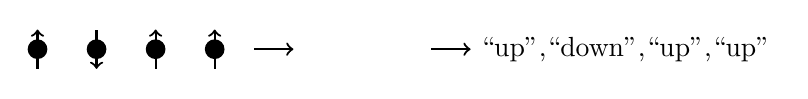
\begin{tikzpicture}[scale=1]      
      \def\x{-4.3}
      \def\y{0.75}
      
      \fill (\x+0.25,\y-0.5) circle [radius=0.125];
      \draw[->, thick] (\x+0.25,\y-0.75) -- (\x+0.25, \y-0.25);
      
      \fill (\x+1,\y-0.5) circle [radius=0.125];
      \draw[<-, thick] (\x+1,\y-0.75) -- (\x+1, \y-0.25);
      
      \fill (\x+1.75,\y-0.5) circle [radius=0.125];
      \draw[->, thick] (\x+1.75,\y-0.75) -- (\x+1.75, \y-0.25);
      
      % \node at (\x+1.75, \y-0.5) {\dots};
      \fill (\x+2.5,\y-0.5) circle [radius=0.125];
      \draw[->, thick] (\x+2.5,\y-0.75) -- (\x+2.5, \y-0.25);
      
      
      \draw[->, thick] (\x+3, \y-0.5) -- (\x+3.5, \y-0.5);
      
      % Outputs
      \draw[->, thick] (\x+5.25, \y-0.5) -- (\x+5.75, \y-0.5);
    \node[right] at (\x+5.75, \y-0.5)  {\text{``up''},\text{``down''},\text{``up''},\text{``up''}};
  \end{tikzpicture}
  \caption{A Stern-Gerlach type device correctly measures the $\mathrm{\sigma_z}$ observable on some input qubits, each in a $\mathrm{\sigma_z}$ eigenstate.}
\end{subfigure}\label{subfig:stern-gerlach-right-way}\\~\\~\\
\begin{subfigure}{0.7\textwidth}
  \drawDeviceUpsideDown{(-4.3+9.5, 0.75-0.5)}{$\mathrm{\sigma_z}$}{0.8}
  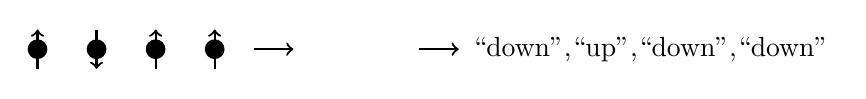
\begin{tikzpicture}[scale=1]    
    \def\x{-4.3}
    \def\y{-0.75}
    
    \fill (\x+0.25,\y-0.5) circle [radius=0.125];
    \draw[->, thick] (\x+0.25,\y-0.75) -- (\x+0.25, \y-0.25);
    
    \fill (\x+1,\y-0.5) circle [radius=0.125];
    \draw[<-, thick] (\x+1.,\y-0.75) -- (\x+1., \y-0.25);
    
    \fill (\x+1.75,\y-0.5) circle [radius=0.125];
    \draw[->, thick] (\x+1.75,\y-0.75) -- (\x+1.75, \y-0.25);
      
    % \node at (\x+1.75, \y-0.5) {\dots};
    
    \fill (\x+2.5,\y-0.5) circle [radius=0.125];
    \draw[->, thick] (\x+2.5,\y-0.75) -- (\x+2.5, \y-0.25);
    
    
    \draw[->, thick] (\x+3, \y-0.5) -- (\x+3.5, \y-0.5);
    
    % Outputs
    \draw[->, thick] (\x+5.1, \y-0.5) -- (\x+5.6, \y-0.5);
    \node[right] at (\x+5.65, \y-0.5)  {\text{``down''},\text{``up''},\text{``down''},\text{``down''}};
    %}
    %\only<3>{
    %  \draw[->,black,thick, font=\bfseries] (\x+2.5, \y+0.75) node[left] {$R_g$} -- (\x+3.5,\y-0.05);
    %  \draw[->,black,thick, font=\bfseries] (\x+8, \y+0.75) node[right] {$f_g$} -- (\x+7,\y-0.05);
    %}
    
  \end{tikzpicture}
  \caption{Rotating the device 180 degrees reverses the output.}
  \end{subfigure}
  \caption{The group $\{0,1\}$ with addition modulo $2$, with the group representation implementing ``flipping the measuring upside-down'', action $f_g:h\mapsto gh$, and the observable $\mathrm{\sigma_z}$ form a system of covariance.}\label{fig:simple-system-of-covariance}
\end{figure}


An application of Wigner's theorem~\cites{wigner1931}{wigner1960} shows that the representation must be of the form
\begin{align}
  R_g:A\mapsto U_g A U_g^*,
\end{align}
where the $U_g$ are either unitary or anti-unitary operators on $\hcal$. Since anti-unitary operators, and anti-linear operators in general, are much less common than their linear counterparts in the quantum information and foundation literature we note the following example, a map $K:\Cx^n\to\Cx^n$ provided by fixing an orthonormal basis $B = \ket{0}\ldots \ket{n-1}$, and defining
\begin{align}
  K: \ket{\varphi} \mapsto \sum_i \braket{i}{\varphi}^* \ket{i},
\end{align}
which differs from a definition of the identity operator only by the complex conjugate. The resulting map is not, of course, independent of the basis chosen, however, for any two anti-unitary maps $K, K^\prime$ there exists a unitary $U$ such that
\begin{align}
  K^\prime = U K,
\end{align}
so a single anti-unitary, combined with the familiar structure of the unitary operators, suffices to explore the space of anti-unitaries~\cite{wigner-antiunitary-1960}.

Covariant quantum observables were introduced by Davies \cite{DAVIES1970318}, using the language of general quantum instruments rather than POVMs, and were already being used in the study of uncertainty by Holevo in 1978 \cite{HOLEVO1979385}. Special cases which have been studied in the literature are covariant symmetric informationally complete-POVMS (SIC-POVMs) \cites{doi:10.1063/1.1896384}{doi:10.1063/1.1737053} and extreme covariant POVMs \cites{doi:10.1063/1.2940328}{doi:10.1063/1.3668317}{doi:10.1063/1.1806262}{erkka-thesis}. Covariance has been employed in the study of measurement uncertainty for angular momentum observables \cite{dsw-meas-ur-ang-mom}, number and angle \cite{sharp-ur-num-angle}, and general phase spaces \cite{Werner2016}.


% For the most part we will deal only with probability spaces where the outcome set is $\Omega\subseteq\R$, in this case we can define the variance of a probability measure $\mu$
% \begin{align}
%   \var{\mu} \defeq \inf_{x_0\in\R}\int_\Omega (x-x_0)^2 d\mu(x),
% \end{align}
% similarly where $\ope$ is a POVM with outcome set a subset of the reals we define
% \begin{align}
%   \var[\rho]{\ope} \defeq \var{\ope_\rho}.
% \end{align}
% Where it makes the text simpler we may use a self-adjoint operator in place of a POVM in such formulae, in these cases we take the measure to be the spectral measure of the operator.

The time evolution will be given by quantum channels, those linear maps from the trace-class operators on one Hilbert space to the trace-class operators on another which preserve the trace, and are completely positive. A corollary of Stinespring's Theorem \ref{thm:stinespring} states that the completely positive maps from a Banach space $\ucal\subseteq\bops[\hcal]$ to $\bops[\mathcal{K}]$ are exactly those which may be written in the form
\begin{align}
  \Phi(\rho) = \tr{U \rho\otimes\rho_0 U^*}[\hcal_0],
\end{align}
where $\hcal_0$ is a Hilbert space and $\rho_0$ is a quantum state in $H_0$. One may, alternatively, consider the quantum state to be unchanging and allow the observables to evolve. This ``Heisenberg picture'' (in contrast to the former ``Schr\"odinger picture'') is furnished by the dual map and is sometimes more convenient.

The dynamics of a perfectly isolated quantum system are reversible, using Wigner's theorem it is possible to show that the bijective channels are those of the form
\begin{align}
  \Phi:\rho&\mapsto U\rho U^*\\
  \Phi^*:E(X)&\mapsto U^* E(X) U,
\end{align}
where $U:\hcal\to\hcal$ is a unitary or anti-unitary map, (see \cite{wigner1960} for a translation of the original work \cite{wigner1931}, or \cite{bargmann1964-wigner} for a detailed proof). The time evolution of quantum mechanics is given by the unitary case, although the anti-unitary operators will be useful in section \ref{chap:cov-meas-ur} when we consider observables symmetric under the action of a group with a representation consisting of both unitary and anti-unitary maps.

% We will occasionally be interested in the state of a system \emph{after} the measurement of an observable. This is formulated in the language of quantum instruments, we will use the Schr\"odinger picture of the evolution of states, although again, one can employ the dual map to obtain the Heisenberg picture. Given a  measurable set $(\Omega, \fcal)$ a \emph{quantum instrument} is map $\mathfrak{I}:\fcal\mapsto \bops[\trops[\hcal]][\trops[\kcal]]$ with the properties
% \begin{enumerate}
%   \item $\mathfrak{I}(X)$ is completely positive, $\forall X\in\fcal$;
%   \item $0\leq \tr{\mathfrak{I}(X)(T)} \leq 1$, $\forall X\in\fcal$ and $T\in\dops[\hcal]$;
%   \item $\tr{\mathfrak{J}(\Omega)(T)} = \tr{T}$, $\forall T\in\trops[\hcal]$;
%   \item $\mathfrak{J}(\bigcup_{i=1}^\infty X_i)(T) = \sum_{i=1}^\infty \mathfrak{J}(X_i)(T)$, $\forall T\in\dops[\hcal]$, and all disjoint sequences $(X_i)_{i=1}^\infty$ where the series converges in trace-norm.
% \end{enumerate}
% We associate $\mathfrak{I}$ with an observable $F$ by the formula
% \begin{align}
%   \tr{F(X)\rho} = \tr{\mathfrak{J}(X)(\rho)},
% \end{align}
% for all $\rho\in\dops[\hcal]$ and all $X\in\fcal$. Every instrument defines a unique observable by this formula, conversely any observable $F$ may be associated with infinitely many instruments. If an observable $F$ is measured via an instrument $\mathfrak{I}$, on state $\rho$ then the post measurement state, having observed outcome $X$ is given by the expression
% \begin{align}
%   \frac{\mathfrak{I}(X)(\rho)}{\tr{\mathfrak{I}(X)(\rho)}},
% \end{align}
% where we avoid division by zero by noting that the probability of observing an outcome $X$ with $\tr{\mathfrak{I}(X)(\rho)} = 0$ is $0$.

\section{Comparing measures and observables}
\label{sec:comp-measures-and-dists}

The textbook description of quantum uncertainty (see e.g. \cite{Nielsen-Chuang}) may be summarised as the claim that there exist pairs of quantum observables $\ope$, $\opf$ for which there does not exist any state $\rho$ which makes the induced probability measures $\ope^\rho$ and $\opf^\rho$ simultaneously sharply concentrated. Often this is characterised by a lower bound on some functional of the variances or entropies \cites{MaassenUffink1988}{Wehner_2010} of the two distributions, valid for all quantum states. A slightly broader view is to consider the set
\begin{align}
  \sbuild{\left(\delta(\ope_1^\rho),...,\delta(\ope_n^\rho)\right)}{\rho\in\dops[\hcal]} \subseteq \R^n,
\end{align}
where the $\ope_i$ are observables on $\hcal$ and $\delta$ is a measure of the uncertainty of a probability measure (e.g. \eqref{eqn:prelim-def-variance}, \eqref{eqn:wassersten-variance} or \eqref{eqn:overall-width-defn}). This approach is known as \emph{preparation uncertainty}, since we range over the quantum states (also called preparations).

An alternative facet of quantum uncertainty is called \emph{measurement uncertainty}. This is a consequence of the fact that quantum mechanics contains incompatible observables, that is, there exist pairs (or larger collections) of quantum observables for which there is no joint observable. We can make quantitative the qualitative statement that a family of observables is incompatible by considering the distance of each observable from the corresponding margin of an \emph{approximate joint observable}, in more mathematical language, given $\sbuild{E_i:\fcal_i\to\dops[\hcal]}{i\in 1...n}$, and $\delta$, representing a distance between observables we are interested in the set
\begin{align}
  \sbuild{\left(\delta(E_1, F_1),...,\delta(E_n, F_n)\right)}{F_i:\fcal_i\to\dops[\hcal]  \text{ are all compatible}}.
\end{align}
Loosely, the $E_i$ are a family of target observables that we would like to measure, incompatibility prohibits this, but we want to know how close we can come to approximating them all simultaneously. This situation is depicted in figure \ref{fig:depict-meas-uncertainty}.

To develop the theory of uncertainty, and particularly measurement uncertainty, it is useful to be able to compare probability measures on some space. For example we might want to make the claim that one distribution is ``broader'' than another, or that one of two distributions approximates a third, target distribution, more accurately than the other. Here we introduce the mathematical tools we will use to do this.

In section \ref{chap:cov-meas-ur} we will compare finite-outcome probability distributions using the $L^p$-metric, defined as
\begin{align}
  \label{eqn:lpvar-defn}
  \lPVar{S}{T}[p]&\defeq \left(\sum_{\omega\in\Omega} \abs{S(\omega) - T(\omega)}^p\right)^\frac{1}{p}, \quad 1\leq p < \infty,\\
  \lPVar{S}{T}[\infty] &\defeq \max_{\omega\in\Omega} \abs{S(\omega) - T(\omega)}.
\end{align}
Note here we are considering probability distributions as functions on the outcome set $\Omega$, rather than measures as function on a $\sigma$ algebra over $\Omega$. The former notation is not well suited to measures with infinite outcome sets, but we will employ it extensively in the finite outcome setting. We note the $L^1$ metric is equal to the definition of total variation distance given in the standard references, e.g. \cite{optimal-transport-villani} and \cite{topics-optimal-transport}, which has a natural generalisation to the case of measures with infinite outcomes
\begin{align}
  \lPVar{\mu}{\nu}[1] \defeq \sup_{S\in\fcal}\abs{\mu(S) - \nu(S)}.
\end{align}
The use of the total variation for measurement errors of continuous variables has been criticised in \cite{blw-meas-uncertainty}, on the basis that it is insensitive to any metric on the underlying space. Explicitly, every point measure is at distance $2$ from every other point measure, whereas in a physical context it is often natural to consider point measures corresponding to points which are close together to be similarly close.
A key tool for comparing Borel measures on a metric space $(\mathsf{A}, d)$ is the Wasserstein $\alpha$-metric, using a real parameter $\alpha$ greater than $1$,
\begin{align}
  \ws{\mu,\nu}[\alpha]  \defeq \left(\inf_{\gamma\in\Gamma(\mu,\nu)} \int_{\mathsf{A}\times\mathsf{A}} d(x,y)^\alpha d\gamma(x,y)\right)^\frac{1}{\alpha}.\label{eq:wasserstein-prob-dists}
\end{align}
Here $\Gamma(\mu,\nu)$ is the set of ``couplings'' between $\mu$ and $\nu$, the probability measures on the product space $\mathsf{A}\times\mathsf{A}$, with first margin $\mu$ and second margin $\nu$.

We provide a simple example, computing the Wasserstein $\alpha$distance between two probability distributions on the outcome set $\{-1,1\}$. We let 
\begin{align}
  \mu(1) &= m\\
  \mu(-1) &= 1-m\\
  \nu(1) &= v\\
  \nu(-1) &= 1-v.
\end{align}
An arbitrary probability distribution on the outcome set $\{-1,1\}\times \{-1,1\} = \{(1,1), (1,-1), (-1,1), (-1,-1)\}$ is given by
\begin{align}
  p(1,1) &= a\\
  p(1,-1) &= b\\
  p(-1,1) &= c\\
  p(-1,-1) &= 1-a-b-c.
\end{align}
Applying the constraint that $p$ is a coupling of $\mu$ and $\nu$ we obtain
\begin{align}
  p(1,1) + p(1,-1) &= a+b = \mu(1) = m\\
  p(-1,1) + p(-1,-1) &= 1-a-b = \mu(-1) = 1-m\\
  p(1,1) + p(-1,1) &= a+c = \nu(1) = v\\
  p(1,-1) + p(-1,-1) &= 1-a-c = \nu(-1) = 1-v.
\end{align}
We therefore have a family of couplings parameterised by a single real parameter
\begin{align}
  p_a(1,1) &= a\\
  p_a(1,-1) &= m-a\\
  p_a(-1,1) &= v-a\\
  p_a(-1,-1) &= 1+a-m-v,
\end{align}
where positivity requires
\begin{align}
  \max\{0, m+v-1\} \leq a \leq \min\{m,v\}.
\end{align}
Since $\mu$ and $\nu$ are discrete the integral in equation~\ref{eq:wasserstein-prob-dists} becomes a sum and we obtain
\begin{align}
  \ws{\mu,\nu}[\alpha] &= \left(2^\alpha\inf_a\left(p_a(1,-1) + p_a(-1,1)\right)\right)^\frac{1}{\alpha}\\
                       &= 2 \left(\inf_a \left(m+v - 2a\right)\right)^\frac{1}{\alpha}\\
                       &= 2 \abs{m-v}^\frac{1}{\alpha}.
\end{align}
We take the formula for the moments from ref.~\cite{statistical-inference}.
\begin{defn}[Moments]\label{defn:moments}
  For $n\in\N$ the the $n^\text{th}$ moment of a probability measure $\mu:\mathcal{B}(\R)\to [0,1]$, on the reals is defined by the integral
  \begin{align}
    \mu[n] \defeq \int_\R x^n d\mu(x).
  \end{align}
\end{defn}
In general the even moments may be real numbers or positive infinity, whereas the odd moments may be real, positive or negative infinity, or undefined, for example in the case of the Cauchy distribution. In the case where the probability measure is dominated by the familiar Lebesgue measure, that is where there exists a probability density function $p:\R\to[0,1]$ such that
\begin{align}
  \mu(X) = \int_X p(x) dx,
\end{align}
the formula for the moments becomes
\begin{align}
  \mu[n] \defeq \int_\R x^n p(x) dx.
\end{align}

% The moments 
% If $\mu:\mathcal{B}(\R)\to [0,1]$ is a probability measure then we define the 

% can compute the integrals
% \begin{align}
%   I^-(n) &= \int_{X^{-}(n)} (-x)^n d\mu(x),\\
%   I^+(n) &= \int_{X^{+}(n)} x^n d\mu(x),
% \end{align}
% where $X^{+}(n)$, (resp. $X^{-}(n)$) is the subset of $\R$ for which $x^n$ is non-negative, (resp. negative). Both integrands are non-negative and measurable on the regions of integration so both integrals exist, but may be equal to $+\infty$. If at least one integral is finite we define the $n^\text{th}$ moment of $\mu$
% \begin{align}
%   \mu[n] \defeq I^+(n) - I^-(n),
% \end{align}
If the first and second moments of a probability measure exist and are finite then we can define the variance
\begin{align}
  \var{\mu} \defeq \mu[2] - \mu[1]^2, \label{eqn:prelim-def-variance}
\end{align}
which we will use extensively in chapter \ref{chap:low_dim_prep}.

An application of the Wasserstein metric allows a generalisation of the variance to probability distributions with outcome sets which are not subsets of $\R$. To motivate this we consider the simplest case which can not be embedded in the real line; an observable whose outcome set is the set of points on the unit circle $\T$. The circle differs from a closed interval $[a-\pi, a+\pi]$ only by identifying the endpoints and is given the structure of a metric space by defining the quantity
\begin{align}
  d(x_1,x_2) \defeq \min_{n\in \{-1,0,1\}} \abs{x_1 + 2n\pi - x_2},
\end{align}
where the minimisation reflects the fact that two points may be connected by arcs either way around the circle. We show there is no way to define the variance of a probability distribution on the unit circle by considering the uniform distribution, to define the variance one first needs to define a mean, and there is no unique way to assign a mean to the uniform distribution over the circle. Nonetheless, there is a natural sense in which some distributions on $\T$ are more concentrated than others. For a metric space $(\mathsf{A}, d)$, and Borel probability measure $\mu$ we define
\begin{align}
  \wsDev{\mu}[\alpha] \defeq \inf_{x_0\in\mathsf{A}} \ws{\mu, \delta_{x_0}}[\alpha], \label{eqn:wassersten-variance}
\end{align}
where $\delta_{x_0}$ is a point measure supported at $x_0$. If $\mu$ is a probability measure on the Borel sets of $\R$, with the standard topology, for which the mean and variance exist, it is easy to see that when $\alpha=2$, the infimum in \eqref{eqn:wassersten-variance} is attained where $x_0$ equals the mean and that $\wsDev{\mu}[2]$ equals the standard deviation of $\mu$. Similarly, $\wsDev{\mu}[1]$ is the absolute deviation, and the infimum is attained at the median. The $\alpha$-deviation appears in \cite{blw-meas-uncertainty}, and was applied in \cite{sharp-ur-num-angle} to the case of covariant number and phase observables. Note that the only coupling between a measure and a point measure is the product measure, so the formula \eqref{eq:wasserstein-prob-dists} simplifies substantially in this case
\begin{align}
  \wsDev{\mu}[\alpha] = \inf_{x_0\in\mathsf{A}} \left(\int_{\mathsf{A}} d(x,x_0)^\alpha d\mu(x)\right)^\frac{1}{\alpha}.
\end{align}
The Wasserstein metric was used in the context of quantum uncertainty by Busch, Lahti and Werner in \cite{PhysRevLett.111.160405}, with a focus on the case of canonically covariant observables $\ope^Q$ and $\ope^P$, and restricted to $\alpha=2$. In \cite{blw-meas-uncertainty} the same authors generalised this approach to consider arbitrary $\alpha$. In these papers the authors considered both the supremum of the Wasserstein metric over all states, called the metric error, and a quantity called the calibration error. For observables for which there are states which make the induced probability distributions deterministic the calibration error is given by the maximum over those states. In general an observable may not induce a deterministic probability distribution in any state, so the calibration error is given by a limiting procedure
\begin{align}
  \calibError{F}{E}{\alpha}[\varepsilon] &\defeq \sup_{\rho,x} \sbuild{\ws{F^\rho,\delta_{x}}[\alpha]}{\ws{E^\rho,\delta_{x}}[\alpha]}\\
  \calibError{F}{E}{\alpha} &\defeq \lim_{\varepsilon\to 0} \calibError{F}{E}{\alpha}[\varepsilon]  
\end{align}
The overall width is a natural measure of the broadness of a probability measure on the reals. Given $\varepsilon\in (0,1)$ we define
\begin{align}
  \width{\mu}{\varepsilon} \defeq \inf_{a,b\in\R} \sbuild{\abs{a-b}}{\mu([a,b])\geq 1-\varepsilon}, \label{eqn:overall-width-defn}
\end{align}
the set bounded below by zero, and non-empty since for any $\varepsilon$ there is an $n$ large enough such that $\mu([-n,n])\geq 1-\varepsilon$ so this quantity is a real number. The overall width has been studied in the context of timelimited and bandlimited functions in \cite{6773660}, in the quantum mechanical literature by Uffink \cite{ufink-thesis}, Busch et. al.~\cite{BUSCH2007155} and Miyadera~\cite{doi:10.1063/1.3614503}.

Entropic quantities have also been used to study quantum uncertainty, although the set of quantities which are called ``entropies'' is large, for our purposes it suffices to consider the R\'enyi $\alpha$-entropies~\cite{renyi1961}. For a probability distribution on a finite set, these are given by
\begin{align}
  H_\alpha(P) = \frac{1}{1-\alpha} \log{\sum_i P(i)^\alpha}.
\end{align}
The R{\'e}nyi entropies are \emph{Schur concave} as functions of the probability distribution. We write $P \prec Q$ if $P$ may be written as a convex combination of permutations of $Q$, and say $Q$ majorizes $P$ in this case. Schur concavity is the property that
\begin{align}
  P\prec Q \implies H_\alpha(P) \geq H_\alpha(Q),
\end{align}
roughly speaking the entropy will be larger for a more ``spread out'' distribution than a more concentrated one.

Given a distance measure $\delta$ on probability distributions one can define a distance measure on quantum observables by choosing a relevant set of states $S\subseteq \dops[\hcal]$ and setting
\begin{align}
  \delta_S(E, F) \defeq \sup_{\rho\in S} \delta(E^\rho, F^\rho),
\end{align}
of course the choice of the set $S$ is highly significant and the appropriate choice will depend on the application. In general choosing a larger $S$ makes the test more stringent. To make a classical analogy one would be unconvinced by a clock sold as being able to tell one time (per day) highly accurately, but a clock sold as being able to tell \emph{all} times with error less than some bound is more convincing. Indeed this analogy can be made quite precise, given any two observables $E$ and $F$ one can perfectly reproduce the statistics $E^\rho$, and $F^\rho$ in a fixed state $\rho$ with the (trivial) observable
\begin{align}
  J: (A,B) \mapsto E^\rho(A) F^\rho(B) I.
\end{align}
In chapter \ref{chap:cov-meas-ur} the set $S$ will be the whole state-space, and the distance measure on probability distributions will be the  $\alpha$-deviation given in \eqref{eqn:wassersten-variance}. In general the choice of distance on the probability measures is also application dependent, but we note that if $\delta$ is a metric on the space of probability distributions, and $S$ spans $\dops{\hcal}$ then $\delta_S$ is a metric on the observables. Measuring differences between observables in terms of the outcome statistics was proposed by Ludwig \cite{ludwig-foundations-of-qm}, although the formulation of measurement uncertainty we are interested in in this thesis was introduced by Busch, Lahti and Werner \cite{blw-meas-uncertainty}.

\begin{subappendices}
\section{Example of a non-basis independent ``trace''}\label{app:bad-sum-is-bad}
Consider an infinite dimensional Hilbert space spanned by basis vectors $\left\{\ket{e_k}\middle|k\in\N\right\}$. Let $Z$ be the operator acting as
\begin{align}
  Z\ket{e_{2n}} &= \ket{e_{2n}}\\
  Z\ket{e_{2n+1}} &= -\ket{e_{2n+1}},
\end{align}
effectively the direct sum of Pauli-z operators acting in two dimensional subspaces. For $k\in\N$ define the operators $U_{k\theta}$ acting as rotations around the $y$ axis in the $k^\text{th}$ two dimensional subspace, and the identity outside
\begin{align}
  U_{k\theta} \ket{e_{2k}} &= \cos(\theta) \ket{e_{2k}} + \sin(\theta)\ket{e_{2k+1}}\\
  U_{k\theta} \ket{e_{2k+1}} &= -\sin(\theta) \ket{e_{2k}} + \cos(\theta)\ket{e_{2k+1}}\\
  U_{k\theta} \ket{e_k} &= \ket{e_j},                            
\end{align}
where $j\neq 2k, 2k+1$, then 
\begin{align}
  \braket{U_{k\theta}e_{2k}}{ZU_{k,\theta}e_{2k}} &= \cos^2(\theta) - \sin^2(\theta)\\
  \braket{U_{k\theta}e_{2k+1}}{ZU_{k,\theta}e_{2k+1}} &= -\cos^2(\theta) + \sin^2(\theta).
\end{align}
We choose $\theta_k$ such that 
\begin{align}
  \braket{U_{k\theta_k}e_{2k}}{ZU_{k,\theta_k}e_{2k}} = \frac{1}{k+1} = -\braket{U_{k\theta_k}e_{2k+1}}{ZU_{k,\theta_k}e_{2k+1}}.
\end{align}
If the basis $\left\{\ket{\phi_k}\middle|k\in\N\right\}$ is chosen such that 
\begin{align}
  \ket{\phi_{2k}} &= U_{k,\theta_k}e_{2k}\\
  \ket{\phi_{2k+1}} &= U_{k,\theta_k}e_{2k+1},
\end{align}
then we can rewrite the terms of the series
\begin{align}
  \sum_{k\geq 0} \braket{\phi_k}{Z\phi_k} = \sum_{k>0}\frac{(-1)^{k-1}}{\lfloor k/2\rfloor},
\end{align}
where $\lfloor x\rfloor$ denotes the \emph{floor} of $x$, the largest natural below $x$. It is now easy to see the series converges to zero, but does not converge absolutely. By the Riemann series theorem \cite{Sierpinski1910} this series may be rearranged (by relabelling basis elements) to give any real number as the sum.

\end{subappendices}

% \begin{subappendices}


% \section{Square root of positive operator}

% Let $A\in\posops[\hcal]$ be positive and bounded, without loss of generality we choose $A \leq \opi$, by multiplying by a positive real number if necessary. We choose $B_0 = \opi$, and note that if $X$ is a positive definite (hence invertible) operator, then
% \begin{align}
%   \frac{1}{2}\left( \frac{A}{X} + X \right),
% \end{align}
% is also positive definite

% \end{subappendices}